% !TeX program = xelatex
\documentclass[border=1cm,convert=ghostscript,11pt]{standalone}
\usepackage{fontspec}
\setmainfont{Times New Roman}[Ligatures=Rare]
\usepackage{microtype}
\usepackage{tikz}
\usetikzlibrary{calc}
\begin{document}
	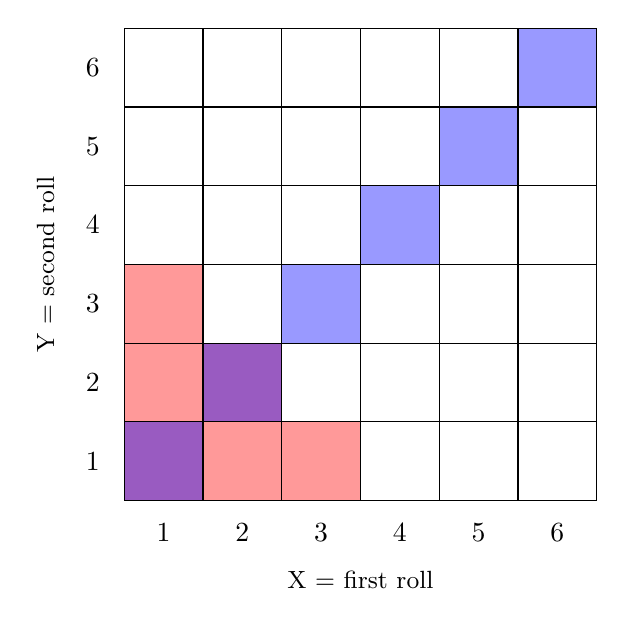
\begin{tikzpicture}
	\foreach \x in {1,...,3} {
		\fill[red!40] (0,\x-1) rectangle (4-\x,\x);
	}
	\foreach \x in {1,...,6} {
		\fill[blue,opacity=.4] (\x-1,\x-1) rectangle (\x,\x);
		\node at (\x-.5,-.4) {\x};
		\node at (-.4,\x-.5) {\x};
	}
	\draw (0,0) grid (6,6);
	\node at (3,-1) {\small X = first roll};
	\node[rotate=90] at (-1,3) {\small Y = second roll};
	\end{tikzpicture} \quad
	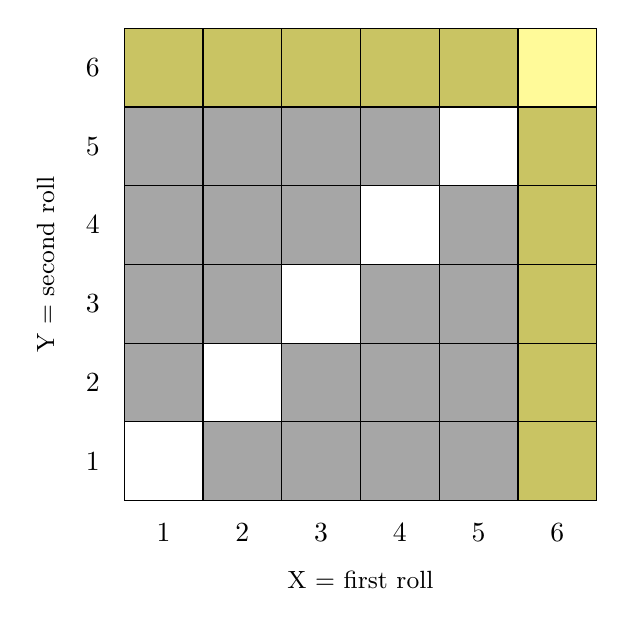
\begin{tikzpicture}
	\foreach \x in {1,...,6} {
		\fill[gray!70] (\x,\x-1) rectangle (6,\x);
		\fill[gray!70] (\x-1,\x) rectangle (\x,6);
		\node at (\x-.5,-.4) {\x};
		\node at (-.4,\x-.5) {\x};
	}
	\fill[yellow,opacity=.4] (0,5) rectangle (6,6);
	\fill[yellow,opacity=.4] (5,0) rectangle (6,5);
	\draw (0,0) grid (6,6);
	\node at (3,-1) {\small X = first roll};
	\node[rotate=90] at (-1,3) {\small Y = second roll};
	\end{tikzpicture}
\end{document}